\documentclass{tufte-handout}

\AtBeginDocument{ \fontsize{16}{20}\selectfont }



\title[Modeling of Wave Propagation]{A Review of Recent Progress in Elastic Waves Propagation Modeling Using Machine Learning Based Methods}

\author[Oscar Rincón-Cardeño]{Oscar Rincón-Cardeño}

\date{August 15, 2024} % without \date command, current date is supplied

%\geometry{showframe} % display margins for debugging page layout
\usepackage{ifxetex}
\ifxetex
  \newcommand{\textls}[2][5]{%
    \begingroup\addfontfeatures{LetterSpace=#1}#2\endgroup
  }
  \renewcommand{\allcapsspacing}[1]{\textls[15]{#1}}
  \renewcommand{\smallcapsspacing}[1]{\textls[10]{#1}}
  \renewcommand{\allcaps}[1]{\textls[15]{\MakeTextUppercase{#1}}}
  \renewcommand{\smallcaps}[1]{\smallcapsspacing{\scshape\MakeTextLowercase{#1}}}
  \renewcommand{\textsc}[1]{\smallcapsspacing{\textsmallcaps{#1}}}
  \usepackage{fontspec}
\fi

\usepackage{graphicx} % allow embedded images
  \setkeys{Gin}{width=\linewidth,totalheight=\textheight,keepaspectratio}
  \graphicspath{{graphics/}} % set of paths to search for images
\usepackage{amsmath}  % extended mathematics
\usepackage{booktabs} % book-quality tables
\usepackage{units}    % non-stacked fractions and better unit spacing
\usepackage{multicol} % multiple column layout facilities
\usepackage{lipsum}   % filler text
\usepackage{fancyvrb} % extended verbatim environments
  \fvset{fontsize=\normalsize}% default font size for fancy-verbatim environments

% Standardize command font styles and environments
\newcommand{\doccmd}[1]{\texttt{\textbackslash#1}}% command name -- adds backslash automatically
\newcommand{\docopt}[1]{\ensuremath{\langle}\textrm{\textit{#1}}\ensuremath{\rangle}}% optional command argument
\newcommand{\docarg}[1]{\textrm{\textit{#1}}}% (required) command argument
\newcommand{\docenv}[1]{\textsf{#1}}% environment name
\newcommand{\docpkg}[1]{\texttt{#1}}% package name
\newcommand{\doccls}[1]{\texttt{#1}}% document class name
\newcommand{\docclsopt}[1]{\texttt{#1}}% document class option name
\newenvironment{docspec}{\begin{quote}\noindent}{\end{quote}}% command specification environment

%------------------------------------
 \usepackage{inputenc}[utf8]

% Keywords command
\providecommand{\keywords}[1]
{
  \small	
  \textbf{{Keywords:}} #1
}

\setmainfont{newbask}[
  Path = ./fonts/,
  UprightFont = *n.ttf,
  BoldItalicFont = *z.ttf,
  BoldFont = *b.ttf,
  ItalicFont = *i.ttf,
  BoldFeatures = {SmallCapsFont = {nbaskervillecapbold}},
  ItalicFeatures = {SmallCapsFont = {lmromancaps10-oblique-webfont}},%newbaskervillecap%lmromancaps10-oblique-webfont
  SmallCapsFont ={lmromancaps}
] 
%\newfontfamily\boldsc{fcmbc8a.pfb}[Path=./Fuentes/]
% Set the math font
\usepackage[italic]{mathastext}
\usepackage{enumitem}
\setlist{noitemsep}
\usepackage{amsmath,amssymb}
\usepackage{xurl}
\usepackage{natbib}
\bibliographystyle{unsrtnat}
\setcitestyle{square,numbers}
\usepackage{xcolor}
\definecolor{newgray}{rgb}{0.3, 0.3, 0.3}

\renewcommand{\citep}[2][]{\textcolor{gray}{(\citeauthor{#2}, \citeyear[#1]{#2})}}
\renewcommand{\citeauthoryear}[2][]{\textcolor{gray}{\citeauthor{#2} (\textcolor{gray}{\citeyear[#1]{#2}})}}

 
\usepackage{hyperref}
\hypersetup{
     colorlinks   = true,
     citecolor    = blue,
     linkcolor = red,
     urlcolor= gray
}

\setcounter{secnumdepth}{1}
%------------------------------------
\begin{document}

\maketitle

\begin{abstract}
\noindent
Numerical modeling has been crucial for addressing problems across various scientific and engineering disciplines that involve partial differential equations. In particular, the wave propagation modeling is one of the areas where intensive scientific computation has been developed. Standard numerical modeling methods demonstrate notable accuracy. However, their computational cost can be significant. Alternative methods based on machine learning have recently emerged showing an adequate balance between computational cost and accuracy when applied to wave propagation problems. In this work, we present a review of machine learning methods that have been developed and used to model elastic wave propagation, with special emphasis on geophysical applications.
\end{abstract}
\keywords{wave propagation, neural networks, deep learning, partial differential equations.}

\section{Introduction}

Wave propagation is a physical phenomenon governed by partial differential equations, which hold significant importance across various applied sciences and engineering fields. However, analytical solutions are not always available for most nonlinear systems, and numerical methods are usually required to approximate the exact solutions. Consequently, these methods have been applied to solve the partial differential equations, achieving the required accuracy \citep{Seriani2020}.

In the field of wave propagation, numerous techniques address wave propagation challenges. Classical methods include finite-difference, finite-element and spectral-element methods \citep{Moczo, virieux_review_2011, Igel2017,komatitsch_introduction_1999,chaljub_spectral-element_2007}. In these approaches, the spatial coordinates are discretized. In the context of mathematical modeling, the primary objective is to ensure that the solution methods are computationally efficient without sacrificing accuracy to capture the physical details inherent to the system. However, standard numerical methods often encounter difficulties when addressing complex problems such as irregular geometries, material changes, and mixed boundary conditions. Therefore, the computational demand associated with many common models in computational mechanics has increased the development of innovative strategies.

Research conducted with the use of machine learning has considerably grown in the late 2010s, owing to advancements in hardware, such as graphic processing units and data storage technologies and the growth of available data. Additionally, the discovery of better training practices for neural networks, and the availability of open-source packages like Tensorflow, PyTorch and JAX \citep{abadi_tensorflow_2016,paszke_pytorch_2019,jax2018github}, as well as the availability of Automatic Differentiation in such packages \citep{paszke_automatic_2017,baydin_automatic_2017}. Particularly, deep learning algorithms offer attractive approximation capabilities for any function by mapping the input features to the output targets in a data-driven manner. A version of the Universal Approximation Theorem conclusively demonstrates that neural networks have the capability to accurately approximate a wide variety of nonlinear functions without any dimensionality constraints \citep{barron_universal_1993}. Additionally, multiple physics-informed neural network methods have been recently proposed \citep{cuomo_scientific_2022}. As a consequence there has been a marked increase in the number of publications associated with neural networks and wave propagation modeling. Figure \ref{dl-wave_propagation-publications} shows the number of document published associated to wave propagation modeling and machine learning. 

\begin{marginfigure}
    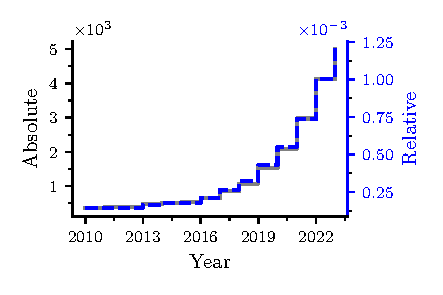
\includegraphics[scale=1]{figs/publications_with_relative.pdf}
    \caption{The growth of literature related to machine learning and wave propagation modeling. Number of publications according to Scopus between 2010 and 2023. The implemented query was: "machine learning" OR "deep learning" OR "neural networks" 
AND "wave propagation" OR "wave equation" 
AND (modeling OR modelling OR model OR simulation).}
    \label{dl-wave_propagation-publications}
\end{marginfigure}

Remarkable reviews have been conducted to address the increasing use of machine learning algorithms across various engineering and scientific disciplines \citep{vadyala_review_2022,deng_physics-informed_2023,lino_current_2023}. Particularly, this review may be of help for researchers with interest into apply these emerging techniques in wave propagation modeling. Due to the extensive areas where wave equation is applied, our aim is to review the recent progress achieved in elastic wave propagation modeling by employing these emerging techniques, specially on geophysics, and the publication time-span studied for those applications was 2014-2024.

This work provides a comprehensive analysis of the advancements made and their impact. While this area can be applied to a wide range of problems, our focus will be limited to the propagation of mechanical waves. The work is organized into the following sections: Section \ref{sec:fordward_inverse_modeling_mechanical_waves} reviews the fundamentals of mechanical wave propagation modeling. Furthermore, in Sections \ref{sec:tnm} and \ref{sec:dl_mwpm}, we identify existing standard and deep learning methods used to solve the wave equation and highlight their strengths and weaknesses in comparison to each other. Additionally, we examine the recent advances in mechanical wave propagation modeling achieved through these methods. Finally, in Section \ref{sec:final_remarks_and_perspectives}, we discuss possible challenges and opportunities.
 
\section{Modeling of Mechanical Wave Propagation}\label{sec:fordward_inverse_modeling_mechanical_waves}
 
A dynamic model, such as the propagation of waves in a medium, describes how a system changes over time. This is different from a static model, which shows how a system is at equilibrium. Dynamic models typically use differential equations to describe how a system evolves. A general formulation of the governing equation of a physical problem can be:

\begin{equation}
D(\boldsymbol{u}(x,t); \lambda) = f(x,t), \quad x \in \Omega, \quad t \in [0, T]\label{eq:pde}
\end{equation}

\

where $D$ denotes the differential operator acting on the solution to the differential equation $u(x,t)$ parameterized by $\lambda$, $f(x, t)$ is a source term. While, $\Omega$ and $\partial\Omega$ denote the spatial domain and its boundary. Equation \ref{eq:pde} can be used to model different systems. We denote the corresponding boundary conditions and the initial condition by:

\begin{equation}
B (u(x, t)) = g(x, t), \quad x \in \partial \Omega, \quad t \in [0, T] 
\end{equation}

\begin{equation}
u(x, 0) = h(x, 0), \quad x \in \Omega
\end{equation}

\

The prescribed initial condition and boundary condition are characterized via $h(x)$ and $g(x, t)$.

Two general approaches when mathematically modeling a system are the inverse and forward problems. The process of determining the causes of a set of observations is known as the inverse problem \citep{Tarantola}, aiming to infer, for example, the properties of a medium based on its reaction to mechanical wave propagation. Since it begins with the effects and then calculates the causes, it is the opposite of a forward problem, which determines the effects based on the causes. In most cases, the inverse problem is formulated by iteratively performing forward modeling to infer the causes that produce a desired effect, making it computationally complex. An schematic representation of the forward and inverse model using numerical methods is shown in Figure \ref{fig:forward_inverse}.

\begin{figure*}[tb!]
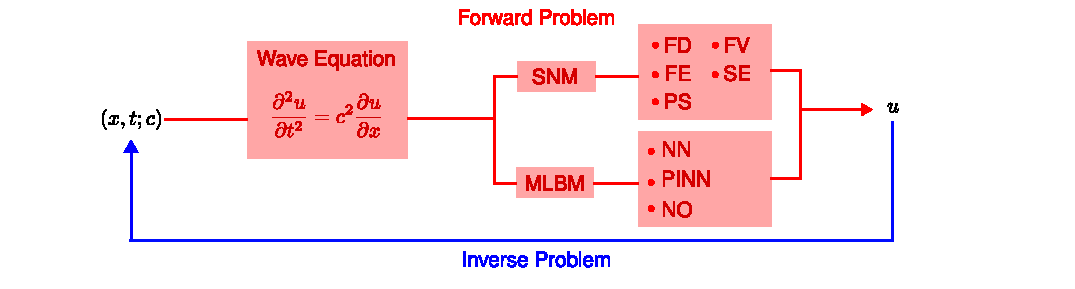
\includegraphics{figs/Forward_Inverse_Modeling_Waves.pdf}
    \caption{Scheme of the forward and inverse problems encountered in solving partial differential equations (PDEs). In the forward scenario, the inputs $(x,\lambda)$ are employed to characterize a model across PDEs. Subsequently, the PDEs are resolved through either standard numerical methods (SNM) or neural networks based methods (MLBM) to derive a solution $u$. Standard numerical methods such as: finite differences (FD), finite elements (FE), pseudo-spectral (PS), finite volumes (FV), and spectral elements (SE). Also, deep learning techniques include, for example, Physics Informed Neural Networks (PINNs), Neural Operator (NO), and Neural Networks (NN). In the case of the inverse problem, the objective is to determine the parameters, for example, the wave speed, $c$ starting from the solution $u$.}
    \label{fig:forward_inverse}
\end{figure*}

Inverse problems are closely tied to simulation, and solving them is crucial for many real-world tasks. Moreover, some complex physical problems require determining the properties of a physical system governed by partial differential equations from observational data, rather than solving them directly to obtain a function that satisfies them \citep{galiounas_battery_2022, ren_seismicnet_2024,mccann_convolutional_2017}. The objective is to estimate a set of latent or unobserved parameters of a system based on real-world observations. Within the framework described by Equation \ref{eq:pde}, the task involves estimating $\lambda$ given $u$. Inversion can be exceedingly challenging since often requires numerous forward simulations to align the predictions of the physical model with the set of observations. 


Wave propagation simulations are essential tools in many areas of geophysics...


The differential equations of interest in this review are those that provide a mathematical description of mechanical wave propagation. We initially consider a continuous medium with a domain $\Omega$ and a boundary $\Gamma$. Denoting by $\mathbf{r}$ the position vector defined at time $t$ within the interval $(0, T)$, where $T > 0$ and $T \in \mathbb{R}$, we introduce:

\[
\begin{aligned}
\hat{\Omega} &= \Omega \cup \Gamma, &\quad
Q_T &= \Omega \times (0,T), &\quad
\Sigma_T &= \Gamma \times (0,T).
\end{aligned}
\]

\

Here, $x_k$ for $k \in \{1, 2, 3\}$ are Cartesian coordinates and $t$ is time. The wave equation problem involves finding a function \( u : \Omega \to \mathbb{R} \) that satisfies the following equations.

Despite being the most elementary among mechanical wave equations, the scalar (acoustic) wave equation is widely used to study seismic waves and in medical applications \citep{moseley_physics-informed_2022, alkhadhr_wave_2023}. The second-order linear wave equation in a homogeneous medium can be expressed as \citep{Carcione2002}:

\begin{equation}
\frac{\partial^2 \boldsymbol{u}(\boldsymbol{x_i}, t)}{\partial t^2} - c^{2} \nabla^2 \boldsymbol{u}(\boldsymbol{x_i}, t) = f(\boldsymbol{x_i}, t) \ ,
\label{acoustic}
\end{equation}

\

where \( \boldsymbol{u}(\boldsymbol{x_i}, t) \) describes the pressure of the seismic waves generated, and \( f(x_i, t) \) is a source term that describes the strength and duration of the source. Another common expression used to describe the propagation of seismic waves, for the case of a heterogeneous isotropic medium, is the elastic wave equation \citep{moseley_fast_2018,lehmann_fourier_2023}. This equation can be expressed as 

\begin{equation}
\rho \frac{\partial^2 \boldsymbol{u}}{\partial t^2} = \nabla \lambda (\nabla \cdot \boldsymbol{u}) + \nabla \mu \left[\nabla \boldsymbol{u} + (\nabla \boldsymbol{u})^T\right] + (\lambda + 2\mu) \nabla (\nabla \cdot \boldsymbol{u}) - \mu \nabla \times \nabla \times \boldsymbol{u} \ ,
\label{elastic}
\end{equation}

where $\rho$ is the material density, $\boldsymbol{u}$ is the displacement vector, and $\lambda, \mu$ are the Lamé parameters characterizing the material.


\section{Standard Numerical Methods to Model Wave Equation}\label{sec:tnm}

In the past decades various numerical methods have been proposed to solve physics systems by partial differential equations such as the wave equation. The finite-difference method is among the most popular to solve partial differential equations, and particularly the wave equation. A complete review of the finite-differences method applied to wave propagation can be found the \citeauthoryear{Moczo2014}. Partial derivatives are approximated by discrete operators involving differences between adjacent grid points. The finite difference method suits for tackling issues related to simple geometric structures. In contrast, the finite element method offers more grid flexibility, facilitating the handling of intricate geometric boundaries.

In wave propagation simulations, the partial differential equations are typically discretized on a staggered grid \citep{madariaga_dynamics_1976,Virieux1986}. This approach facilitates the resolution of the rupture propagation problem. Particularly an approach was proposed in the work of \citeauthoryear{Zhou2021} a finite-difference method with variable-length temporal and spatial operators was proposed to increase the stability and efficiency of the standard method.

\citeauthoryear{liu_simulation_2023} combined a standard staggered-grid, finite-difference approach and the perfectly matched layer absorbing boundary to solve 3D first-order velocity-stress equations of acoustoelasticity to simulate wave propagating.

Finite-element methods are suitable for dealing with intricate shapes and diverse materials because they can use irregular grids. They permit flexibility in size, shape, and approximation order. Nevertheless, a drawback is their high demand for computing power. This methodology involves the transformation of the problem at hand into a system of linear equations utilizing the weak formulation of the pertinent differential equation. This transformation is facilitated by employing an interpolation basis comprised of polynomials defined over disjoint domains, commonly referred to as elements.

Popular open-source software is available to apply numerical methods for solving the wave equation. FEniCS, proposed by \citeauthoryear{FEniCS}, offers a computing platform specifically designed for solving partial differential equations using the finite elements method. Specializing in seismic wave propagation and full waveform imaging, SPECFEM is widely used in simulations implemented in Fortran \citep{dimitri_komatitsch_2023_10415228,komatitsch_2024_10823181}. Similarly, but using finite differences, the modeling the fortran library SEISMIC\_CPML \citep{komatitsch_unsplit_2007} is also available. In general, these implementations of standard methods have enabled effective simulations of the wave equation. 

A significant difficulty in using standard methods for wave propagation simulations is their computational cost. Their accuracy is achieved at the expense of the number of points in the grid. Modeling a complex domain can entail a huge amount of grid points, with the wavefield requiring iterative updates across the entire grid at each time step. Additionally, model evaluation and storage are significantly costly \citeauthoryear{saloma_computational_1993}, and their limited capacity to incorporate measured data into their predictions makes them less ideal for use in inverse problems.

\section{Machine learning Methods to Model Mechanical Wave Propagation}\label{sec:dl_mwpm}

The realm of machine learning has recently displayed promise in its capacity to approximate predictions of physical phenomena. These methods can grasp highly nonlinear physics and offer significantly quicker inference times compared to conventional simulations. Therefore, as an alternative to standard methods deep learning have been employed to apply their capability as universal function approximator \citep{hornik_approximation_1991}.

Neural network based methods are a subset of machine learning, whose models are composed of an artificial neural network with a single or multiple processing layers (Figure \ref{deep_learning_subset_architecture}.A). It have shown potential in overcoming the limitations of multiple approaches in various fields such as computer vision, natural language processing, and genomics \citep{lecun_deep_2015,goodfellow_deep_2016}. The fundamental architecture of a neural network architecture is conformed by an input layer, an output layer, and an arbitrary number of hidden layers. Particularly, in a fully connected neural network, neurons in adjacent layers are connected with each other but neurons within a single layer share no connection (Figure \ref{deep_learning_subset_architecture}.B). Furthermore, neural networks methods have emerged as an attractive tool to augment and complement conventional numerical solvers of partial differential equations, thereby enabling the tackling of challenges across multiple dimensions, scales, and parameterization with the promise of efficiency and precision \citep{blechschmidt_three_2021}. 

\begin{figure*}
    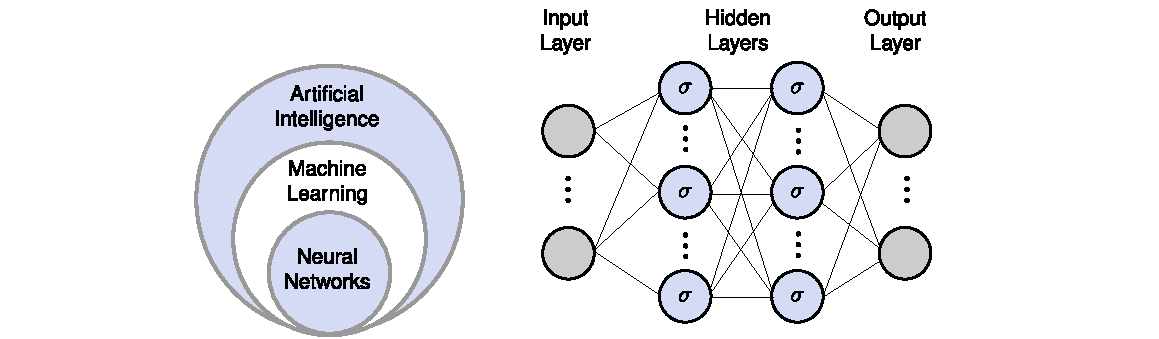
\includegraphics{figs/Artificial_Intelligence_subsets.pdf}
    \caption{Artificial Intelligence subsets. (A) Deep learning as a subset of machine learning and artificial intelligence and (B) basic architecture of artificial neural networks.}    
    \label{deep_learning_subset_architecture}
\end{figure*}

They essentially model the partial differential equation solution by a deep neural network and train the network’s parameters to approximate the solution. Data-driven neural networks methods are capable of directly learning the trajectory of a system of partial differential equations from available data \citep{li_neural_2020,li_fourier_2021}.

One of the most popular types of deep neural networks is known as convolutional neural networks. A convolutional neural network convolves learned features with input data, and uses 2D convolutional layers, making this architecture well suited to processing 2D data, such as images.

 All these approaches employ machine learning algorithms and others such as support vector machines, random forests, Gaussian processes have been also applied to model physical systems. However, they are implemented mainly as black-box tools. The constructed neural network can be thought of being ignorant of the mathematical description of the physical phenomenon. In order to overcome this limitation physics-informed neural networks architectures have been proposed. Where the activation and the loss functions are designed according to the context of the problem.

There has been an increasing interest in leveraging physics-informed neural networks to solve forward and inverse problems where full or partial knowledge of the governing equations is known since the published works of \citeauthoryear{raissi_hidden_2018}, \citeauthoryear{raissi_numerical_2018} and \citeauthoryear{Raissi2019}. Although similar ideas for constraining neural networks using physical laws have been explored in previous studies \citep{lagaris_artificial_1998}. The general principle of physics-informed neural networks is to integrate deep neural networks and physical laws to learn the underlying consistent dynamics from small or zero labeled data \citep{karniadakis_physics-informed_2021}. As universal approximators, neural networks have the potential to represent any partial differential equation. This capability eliminates the need for the discretization step, thereby avoiding discretization-based physics errors as well. 


\begin{figure*}
    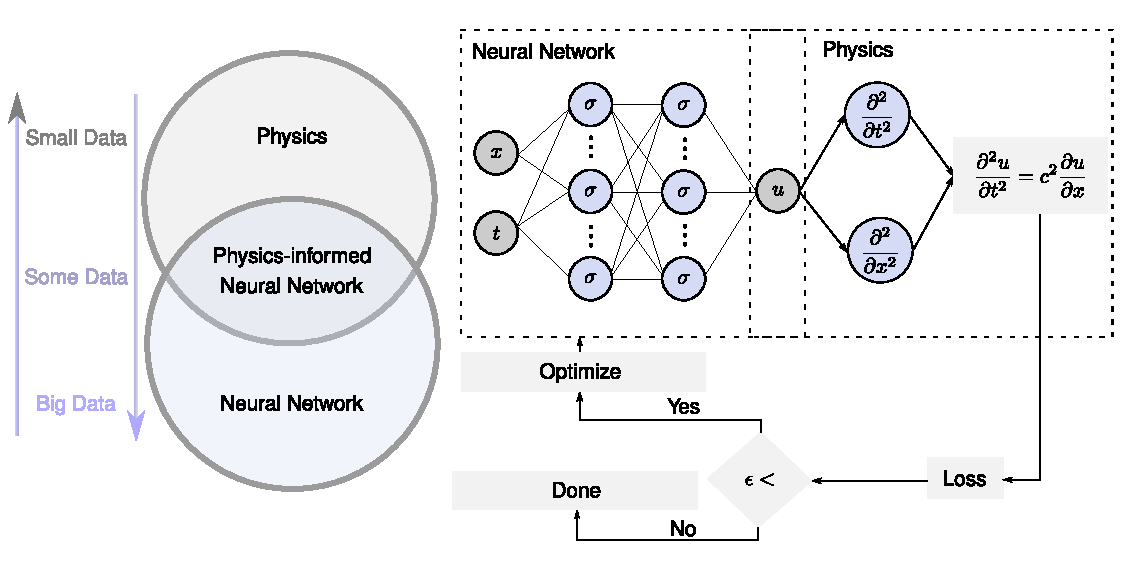
\includegraphics{figs/Escheme_PINN_waves.pdf}
    \caption{Physics-informed neural networks scheme applied to the wave equation.}
    \label{deep_learning_subset_architecture}
\end{figure*}

Physics-informed neural networks aim to address physical systems governed by the equation

$$
u_{tt} - D[u(t, x); \lambda] = 0,
$$

\

where \(x \in \mathbb{R}^D\) and \(t \in \mathbb{R}\). The expression \(N[u(t, x); \lambda]\) denotes an underlying differential operator that characterizes the physical system, parametrized by \(\lambda\). The function \(u(t, x)\) represents the system's solution. The loss function is of the general form 

$$ L := \beta_{\text{pde}}L_{\text{pde}}(\sigma) + \beta_{\text{ic}}(\sigma) L_{\text{ic}} + \beta_{\text{bc}} L_{\text{bc}}(\sigma) ,$$

where

$$
\begin{aligned}
& \mathcal{L}_{pde}(\boldsymbol{\sigma})=\frac{1}{n_{pde}} \sum_{i=1}^{n_{pde}}\left|u_{tt} - \mathcal{D}\left[\hat{u}\left(t, \boldsymbol{x}_i ; \boldsymbol{\sigma}\right)\right]-f\left(t, \boldsymbol{x}_i\right)\right|^2, \\
& \mathcal{L}_{bc}(\boldsymbol{\sigma})=\frac{1}{n_{bc}} \sum_{i=1}^{n_{bc}}\left|\hat{u}\left(t, \boldsymbol{x}_i ; \boldsymbol{\sigma}\right)-g\left(t, \boldsymbol{x}_i\right)\right|^2, \\
& \mathcal{L}_{ic}(\boldsymbol{\sigma})=\frac{1}{n_{ic}} \sum_{i=1}^{n_{ic}}\left|\hat{u}\left(0, \boldsymbol{x}_i ; \boldsymbol{\sigma}\right)-h\left(t,\boldsymbol{x}_i\right)\right|^2,
\end{aligned}
$$

\

and \( L_{\text{pde}} \) represents the residuals of the PDEs, \( L_{\text{ic}} \) represents the error at the collocation points at the initial time point, and \( L_{\text{bc}} \) represents the error at the collocation points on the boundaries. The coefficients \(\beta_{\text{ic}}\) and \(\beta_{\text{bc}}\) are training hyper-parameters.


\section{Applications}

This section presents the findings from a search focused on how machine learning have been used for modeling elastic wave propagation. The search was mainly conducted by following query was used on the Scopus website as an initial filter:

\begin{verbatim}
"machine learning" OR "deep learning" OR "neural networks" 
AND "wave propagation" OR "wave equation" 
AND (modeling OR modelling OR model OR simulation)
\end{verbatim}

The search aimed to find significant contributions and advancements in modeling elastic wave propagation using machine learning techniques over the past decade. Additionally, the it was complemented by Google Scholar using the same terms, time span, and language. The resulting list was then sorted by relevance, with the analysis limited to the first 50 results from both engines, which were then merged. Finally, since our focus was particularly on geophysical applications, we selected the works whose abstracts indicated relevance to this field. The total number of works that met these conditions was  (see Figure \ref{fig:Escheme_Systematic_Review}).

\begin{figure*}
    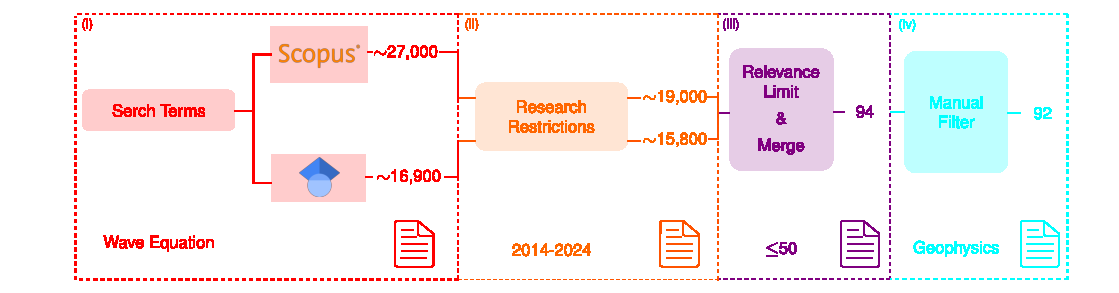
\includegraphics{figs/Escheme_Systematic_Review.pdf}
\caption{Search flowchart and number of publications after each step. During the systematic review process, Scopus and Google Scholar were utilized with the relevant search terms (i), and the research was restricted to works in English and within the time frame of 2013-2024 (ii). The resulting lists were then sorted by relevance and limited to a maximum of 50 entries, with duplicates removed (iii). Finally (iv), a manual filter was applied by reading the titles and abstracts to ensure the publications were pertinent to our chosen field.}
    \label{fig:Escheme_Systematic_Review}
\end{figure*}

%limited the results to articles in the field of earth and planetary sciences. This ensured that the studies were relevant to our research area.

We analyzed different aspects in the selected articles, including the type of partial differential wave equation used, the number of dimensions considered, whether forward, inverse or both modeling approaches were performed, and the specific application within gephysics. The results of this analysis are shown in Figure  .

The introduction of physics-informed neural networks has generated a large amount of work related. For example the work of \citeauthoryear{karimpouli_physics_2020} explores the application of deep learning in geosciences, specifically solving the 1-dimensional time-dependent seismic wave equation. Comparing Gaussian process and physics-informed neural networks, the research shows that these meshless methods, requiring smaller datasets, effectively incorporate physics laws, with the Gaussian process excelling in solution prediction and the neural network proving superior in velocity and density inversion. Their significant potential lies in addressing surrogate modeling and inverse analysis, striking a balance between accuracy and computational efficiency \citep{Song2022}. \citeauthoryear{rash_2022} took a similar approach, but extending to 2D heterogeneous acoustic media, showing that PINNs could invert for ellipsoidal and checkerboard velocity models given the seismic response from sources placed within these models.

%\citep{alkhadhr_modeling_2021}


In \citeauthoryear{moseley_physics-informed_2022}, physics-informed neural networks were successfully applied to the 2D acoustic wave equation, demonstrating satisfactory outcomes in forward wave propagation and full waveform inversions, despite the efficiency of standard methods. Additionally, physics-informed neural networks showcased efficient performance in solving the inverse problem. To train the model, the results of a finite difference model are used. Spatial and temporal coordinates are used as inputs and intra-inputs of the network and their respective wave field as output, which provides uniqueness to the solution. While restricting the solution obtained to the equation used. To test the model, 3 different speed models are used: homogeneous, layered and an irregular model of the Earth's subsoil.

%En \citeauthoryear{moseley_physics-informed_2022}, se aplicaron con éxito redes neuronales basadas en la física a la ecuación de ondas acústicas 2D, demostrando resultados satisfactorios en la propagación directa de ondas y en las inversiones completas de formas de onda, a pesar de la eficiencia de los métodos tradicionales. Además, las redes neuronales basadas en la física mostraron un rendimiento eficiente para resolver el problema inverso.

%Para entrenar el modelo se utilizan los resultados de un modelo en diferencias finitas. Coordenadas espaciales y temporales son usadas como entradas y intradas de la red y su respectivo campo de onda como salida, lo que aporta unicidad a la solución. Mientras que restringe la solución obtenida a la ecuación utilizada.

%Para probar el modelo se utilizan diferentes 3 modelos de velocidad. (i) homogeneo, (ii) en capas y (iii) un modelo irregular del subsuelo terrestre.


Similarly, in \citeauthoryear{ren_seismicnet_2024}, physics-informed neural networks were employed for modeling mechanical wave propagation in semi-infinite domains, showcasing their versatility in forward modeling for seismic wave propagation, without requiring labeled data. These studies collectively highlight the effectiveness of physics-informed neural networks across different wave propagation scenarios.

%\citep{wu_helmholtz-equation_2023}

%The order of differential operators can be effectively reduced by proper integration by-parts, which reduces the required regularity in the (nonlinear) solution space...

%\section{Comparative Study}\label{sec:comparative_analysis}

\section{Final remarks and future perspectives}\label{sec:final_remarks_and_perspectives}

\subsection{Challenges}

One major drawback of these methods is the difficulty of transferring knowledge between different configurations. For example, when solving the wave equation, CNNs and PINNs are trained with a fixed velocity parameter and cannot predict anything for a different velocity value. One of the main challenges in numerically modeling mechanical is associated with the dimensional, given the computational complexity.

Tackling complex high-dimensional systems comes with significant challenges. Despite this, machine learning-based algorithms offer promising prospects for solving partial differential equations, as indicated by studies such as the one by \citeauthoryear{blechschmidt_three_2021}. Most of the applications are implemented in one dimensional or two-dimensional domains. In \citeauthoryear{lehmann_fourier_2023} the Fourier Neural Operator method is applied to model sesimic waves.

Emerging machine learning methods for solving partial differential equations can face difficulties in establishing fair comparison points with standard numerical methods. \citeauthor{mcgreivy_weak_2024} identified two common pitfalls. First, comparing the runtime of a less accurate machine learning method to a more accurate standard numerical method, whereas a fair approach would be to make the comparison under similar accuracy levels. Second, evaluating the standard numerical method that is not suitable for the partial differential equation being solved. These two criteria are essential for properly evaluating performance, but they are not always followed. 

\subsection{Opportunities}

Different extentions of the classical work where PINNs was originally proposed have emerged. \citeauthoryear{kharazmi_variational_2019} proposed variational physics-informed neural networks which instead trained physics-informed neural networks using the variational form of the underlying differential equations. A neural network is still used to approximate the solution of the differential equation, but it is combined with a set of analytical test functions to compute the residual of the variational form of the equation in its physics loss term. Furthermore, they used quadrature points to estimate the corresponding integrals in the variational loss, rather than random collocation points. They found that the variational physics-informed neural networks was able to solve differential equations including Poisson’s equation with similar or better accuracy to a physics-informed neural networks trained using the strong form, whilst requiring less collocation points to train. However, most of these extensions have not yet been applied to wave propagation modeling.

Various open-source frameworks are available for solving partial differential equations using emerging machine learning methods. Python packages such as NeuroDiffEq \citep{chen2020neurodiffeq} and DeepXDE \citep{lu2021deepxde} facilitate the solving of both ordinary and partial differential equations using neural networks as function approximators. A similar implementation in the Julia programming language is NeuralPDE \citep{https://doi.org/10.48550/arxiv.2107.09443}. Additionally, PINNs-Torch \citep{bafghi_pinns-torch_2023} enables the application of Physics-Informed Neural Networks using PyTorch, offering improved performance compared to the original model.

%A single layer Functional Link Artificial Neural Network model was originally introduced by \citeauthoryear{pao_functional_1995}.  

%Application to real seismic data are still scarce. 


\subsection{Summary}

%A summary of the reviewed models are presented in Table \ref{tab:summary}.

% \begin{table}[h]
%     \centering
%     \label{tab:algorithm-pinns}
%     \begin{tabular}{|c|l|c|}
%     \hline
%     Year & Key Contributions & Reference \\ \hline
%     \citeyear{alterman_propagation_1968} &  {First application of a numeric method to elastic wave propagation} & [\citealp{alterman_propagation_1968}]\\ \hline
%     \citeyear{frankel_three-dimensional_1992} &  Extension of the FD method to 3D & [\citealp{frankel_three-dimensional_1992}] \\ \hline
%     \citeyear{lagaris_artificial_1998} &  Artificial neural networks used for solving ordinary and partial differential equations & [\citealp{lagaris_artificial_1998}]\\ \hline
%     \citeyear{abadi_tensorflow_2016} &  Open-source package Tensorflow & [\citealp{abadi_tensorflow_2016}]\\ \hline
%     \citeyear{paszke_pytorch_2019} &  Open-source package Pytorch & [\citealp{paszke_pytorch_2019}]\\ \hline
%     \citeyear{Raissi2019} &  Physics-informed neural networks & [\citealp{Raissi2019}] \\ \hline
%     \citeyear{lehmann_fourier_2023}  & Fourier Neural Operator to 3D seismic waves  & [\citealp{lehmann_fourier_2023}] \\ \hline
%     \end{tabular}
%     \caption[][5.5cm]{Evolution of mechanical wave propagation modeling.}\label{tab:summary}
% \end{table}



It's important to notice that deep learning methods shouldn't be seen as substitutes for standard numerical techniques used in solving partial differential equations. These established methods have been refined over decades and often fulfill the robustness and computational efficiency criteria needed in real-world applications. Also, we focus this review on geophysical applications but the methods revised here can be implemented on other fields, whose physical system modeling require the use of the wave equation. 



\bibliography{refs}

\end{document}


%Here, we describe the wave propagation problem, highlighting recent exciting conceptual advances and methods developments for its study and applications. particularly, seismological wave propagation analysis is mainly considered. Methods used classically for the forward problem of wave propagation, are approached. A comparative analysis of the methods is provided, considering factors such as their accuracy, computational storage, processing requirements, and their capability to account for various parameters essential in a mechanical wave propagation model. Moreover, the machine learning methods informed by physics are analyzed as current possible research path in the wave propagation problem.

% \section{Mathematical modeling of mechanical wave propagation}

% Two possible scientific modeling approaches are the forward and inverse modeling. The process of determining the causes of a set of observations is known as the inverse problem,\cite{Tarantola} aiming to infer, for example, the properties of a medium based on its reaction to mechanical wave propagation. Since it begins with the effects and then calculates the causes, it is the opposite of a forward problem, which determines the effects based on the causes. In most cases, the inverse problem is formulated by iteratively performing forward modeling to infer the causes that produce a desired effect. Forward modeling can be described mathematically as:

% \begin{equation}
% u = \mathcal{F}(x; \lambda),
% \label{eq:forward}
% \end{equation}

% where \(x,\lambda\) is a set of input conditions of the system, \(\mathcal{F}\) defines a physical model of the system, and \(u\) is a set of resulting properties of the system given \(\mathcal{F}\) and \(x,k\). For various systems, forward modeling aims to solve a set of differential equations. The system can be described by

% \begin{equation}
% \begin{aligned}
% D[u(x); \lambda] &= f(x), & \quad x &\in \Omega,\\
% B_k[u(x)] &= g_k(x), & \quad x &\in \Gamma_k \subset \partial\Omega,
% \end{aligned}
% \end{equation}

% for $k = 1, 2, ..., n_b,$ where $D$ is a differential operator, $B_k$ is a set of boundary operators, $u \in \mathbb{R}^{d}$ is the solution to the differential equation, and $f(x)$ is a forcing term. Inverse problems are closely tied to simulation, and solving them is crucial for many real-world tasks. The objective is to estimate a set of latent or unobserved parameters of a system based on real-world observations. Within the framework described by Equation \ref{eq:forward}, the task involves estimating a given $b$. Inversion can be exceedingly challenging since often requires numerous forward simulations to align the predictions of the physical model with the set of observations.


% The set of partial differential equations considered in this work are those who establish a mathematical description of the mechanical wave propagation. Initially, a continuous medium with a domain $\Omega$ and a boundary $\Gamma$ is considered. Denoting by $\mathbf{r}$ the position vector defined at time $ t $ within the interval $(0, T)$, where $ T > 0 $ and $ T \in \mathbb{R} $, we introduce:

% $$
% \begin{aligned}
% \hat{\Omega} &= \Omega \cup \Gamma, &\quad
% Q_T &= \Omega \times (0,T), &\quad
% \sum_T &= \Gamma \times (0,T).
% \end{aligned}
% $$

% Here $x_k$; $k  \in {1, 2, 3}$ are Cartesian coordinates and $t$ is time. The displacement vector is:

% \begin{equation*}
% u(r,t) = [u_1(r,t), \tilde{u}(r,t), u_3(r,t)] \in \mathbb{R}^3 \times [0, T] \times \mathbb{R}; \quad i = 1, 2, 3
% \end{equation*}


% Let $\varepsilon_{ij}$ denote the strain tensor, defined as $\varepsilon_{ij} = \frac{1}{2} \left( \frac{\partial u_i}{\partial x_j} + \frac{\partial u_j}{\partial x_i} \right)$, where $i, j \in {1, 2, 3}$, and $\sigma_{ij}$ represents the stress tensor. The displacement–stress formulation for isotropic media is given by:

% \begin{equation}
% \rho \frac{\partial^2 u_i}{\partial t^2} - \frac{\partial \sigma_{ij}}{\partial x_j} - f_i = 0
% \label{displacement-stress}
% \end{equation}


% where $\rho(x_i)$ is the density in a spatial coordinate ($x_1$, $x_2$, $x_3$).the stress--strain relation can be written using Lam\'e constants $\lambda$ and $\mu$ in the form $\sigma_{ij} = \lambda \varepsilon_{kk} \delta_{ij} + 2\mu \varepsilon_{ij}$. Replacing the displacement by its time derivative, the velocity vector, $v_i = \frac{\partial u_i}{\partial t}$ in equation  \ref{displacement-stress}:\\

% \begin{equation}
% \rho \frac{\partial v_i}{\partial t} - \frac{\partial \sigma_{ij}}{\partial x_j} - f_i = 0
% \label{velocity-stress}
% \end{equation}

% which is known as the velocity-stress formulation. In the uni-dimensional case, of a homogeneous medium, the equation \ref{displacement-stress} simplifies (omitting the force term):

% \begin{equation}
% \rho \frac{\partial^2 u_i}{\partial t^2} - c^{2} \frac{\partial \sigma_{ij}}{\partial x_j} - f_i = 0 \ .
% \label{scalar}
% \end{equation}

% Particularly, the 2D the constant-density acoustic wave equation is given by


% \begin{equation}
% \rho \frac{\partial^2 u_2}{\partial t^2} - c^{2} \frac{\partial \sigma_{ij}}{\partial x_j} - f_i = 0 \ .
% \label{acustic}
% \end{equation}

% The upcoming sections outline the prevailing methodologies widely utilized for both forward and inverse modeling, accompanied by notable advancements associated with them. An schematic representation of the forward and inverse model is shown in Figure \ref{fig:forward_inverse}.

% \begin{figure*}
%     \centering    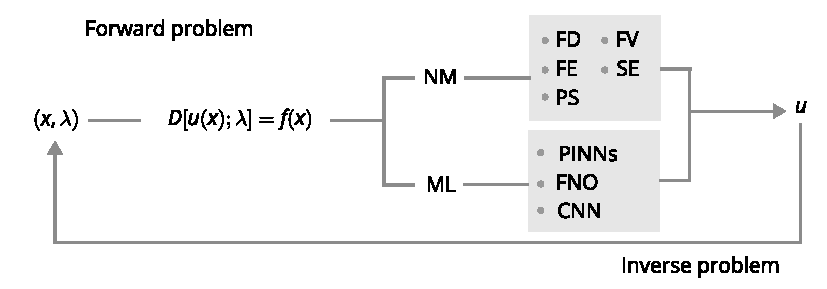
\includegraphics{figs/forward_inverse.pdf}
%     \caption{Scheme of the forward and inverse problems encountered in solving partial differential equations (PDEs). In the forward scenario, the inputs $(x,\lambda)$ are employed to characterize a model across PDEs. Subsequently, the PDEs are resolved through either numerical methods (NM) or machine learning (ML) to derive a solution $u$. Numerical methods encompass finite differences (FD), finite elements (FE), pseudo-spectral (PS), finite volumes (FV), and spectral elements (SE). Machine learning techniques include Physics Informed Neural Networks (PINNs), Fourier Neural Operator (FNO), and Convolutional Neural Networks (CNN). In the case of the inverse problem, the objective is to determine the parameters $(x,\lambda)$ starting from the solution $u$.}
%     \label{fig:forward_inverse}
% \end{figure*}

% \section{Numerical methods}

%  The finite-difference method is among the most popular to solve partial differential equations, and particularly the wave equation. A complete review of the finite-differences method applied to wave propagation can be found the \citet{Moczo2014} and \citet{Seriani2020}. Partial derivatives are approximated by discrete operators involving differences between adjacent grid points. The derivative of a function $f$ is defined as:\\

% \begin{center}
% $
% \frac{df}{dx} = \lim_{dx \rightarrow 0} \frac{f(x + dx)-f(x)}{dx}
% $ , $
% \frac{df}{dx} = \lim_{dx \rightarrow 0} \frac{f(x + dx)-f(x -dx)}{2dx}
% $ or $
% \frac{df}{dx} = \lim_{dx \rightarrow 0} \frac{f(x)-f(x -dx)}{2dx} \ .
% $
% \end{center}


% Considering the Taylor series expansion:



% Then, the approximation schemes of finite-difference derivative, using the Taylor series expansion, are:\\

% \begin{center}
% $
% \frac{df}{dx}^{+} \approx \frac{f(x + dx)-f(x)}{dx}
% $ , $
% \frac{df}{dx}^{c} \approx  \frac{f(x + dx)-f(x -dx)}{2dx}
% $ and $
% \frac{df}{dx}^{-} \approx \frac{f(x)-f(x -dx)}{2dx}
% $
% \end{center}

% Also, the second-order approximation:\

% $$
% \frac{d^{2}f}{dx^{2}} \approx \frac{f(x+dx)-2f(x)+f(x -dx)}{dx} \ .  
% $$

% \

% The following notation is considered for the discrete case of spatial and temporal variables:\

% $$
% u(x,t) \rightarrow u_{j}^{n}
% $$

% \


%  which is also called an \emph{structured grid}. Thus, equation \ref{scalar} can be expressed as:\\

%  $$
% \frac{u_{j}^{n+1} - 2 u_{j}^{n} + u_{j}^{n-1}}{dt^2} = c_{j}^2 \left[ \frac{u_{j}^{n+1} - 2 u_{j}^{n} + u_{j}^{n-1}}{dx^2} \right]  + s_{j}^n
%  $$

% then,

% $$
% u_{j}^{n+1} = \left( c_{j} \frac{dt}{dx} \right)^2 \left[ u_{j+1}^{n} - 2 u_{j}^{n} + u_{j-1}^{n}\right] + 2 u_{j}^{n} - u_{j}^{n-1} + dt^{2} s_{j}^{n}
% $$


% \


% To model this case, a source point is considered, as

% $$
% s(x, t) = \delta(x - x_s) \cdot f(t)
% $$

% Finite-difference methods fall into two broad categories: explicit and implicit. Explicit schemes for simulating the wave equation determine the motion at a spatial location at a future time exclusively from the motion already calculated for previous times. On the other hand, implicit schemes simultaneously determine the motion at all spatial locations at a future time from known values at previous times using a matrix inversion technique.

%In wave propagation simulations, the partial differential equations are typically discretized on a staggered grid \cite{Virieux1986}. This approach facilitates the resolution of the rupture propagation problem. Particularly an approach was proposed in the work of \citet{Zhou2021} a finite-difference method with variable-length temporal and spatial operators was proposed to increase the stability and efficiency of the traditional method.

%\citet{liu_simulation_2023} combined a standard staggered-grid (SSG), finite-difference (FD) approach and the perfectly matched layer (PML) absorbing boundary to solve 3D first-order velocity-stress equations of acoustoelasticity to simulate wave propagating.

% %----------------------------
% \subsection{Pseudo-spectral method formulation}



 
% %----------------------------
% \subsection{Finite-elements method formulation}


% Finite-element methods are suitable for dealing with intricate shapes and diverse materials because they can use irregular grids. They permit flexibility in size, shape, and approximation order. Nevertheless, a drawback is their high demand for computing power. This methodology involves the transformation of the problem at hand into a system of linear equations utilizing the weak formulation of the pertinent differential equation. This transformation is facilitated by employing an interpolation basis comprised of polynomials defined over disjoint domains, commonly referred to as elements.\\

% The finite-element discretization technique, usually denoted as the semidiscrete Galerkin
% formulation, reduces the seismic modeling problem to the following system of second-order, linear, ordinary differential equations:


% \begin{align}
% M\ddot{u} + K u &= \hat{f} \quad \text{for } t \in (0, T) \notag\\
% u(0) &= u_0 \label{fd-formulation-no-damption}\\
% \dot{u}(0) &= \dot{u}_0 \notag
% \end{align}

% where $M$ is the mass matrix, $K$ is the stiffness matrix, $f$ is the load vector and $u$ is the displacement vector.

% One of the problems arising in numerically modeling wave propagation on the earth is the
% need to use a bounded domain which generates undesired reflections. One way to avoid these
% artifacts is to use a very large domain, but this solution is in practice prevented because it requires huge computer storage. To eliminate unwanted reflections we introduce a damping term $A(x,y,z) u$ for $i = 1,2,3$ in differential equation \ref{fd-formulation-no-damption} which is defined only on a boundary layer surrounding the domain. This method can be very accurate but one needs to adjust the damping term.
% The semidiscrete Galerkin formulation, including the damping term, is

% \begin{align}
% M\ddot{u} + C u + K u &= \hat{f} \quad \text{for } t \in (0, T) \notag\\
% u(0) &= u_0 \\
% \dot{u}(0) &= \dot{u}_0 \notag
% \end{align}

% where the damping matrix $C$ is also sparse, symmetric and positive-definite.

% SolidsPy, an open-source software developed by \citet{solidspy}, employs finite element analysis to tackle 2D elasticity problems. It serves as a valuable tool for researchers in computational mechanics and students in Computational Modeling courses, while also finding applications in graduate courses introducing the Finite Element Method. Similarly, FEniCS, proposed by \citet{FEniCS}, offers a computing platform specifically designed for solving partial differential equations using the finite element method.

% \section{Physics-informed machine learning}

%  In recent years, machine learning methods have emerged as an attractive tool to enrich and complement traditional methods, thus allowing challenges to be addressed on multiple dimensions, scales and parameterizations with the promise of efficiency and precision. For example, researchers have explored the Fourier Neural Operator for both forward and inverse analysis of the 2D acoustic wave equation. However, these studies depend on extensive sets of high-quality labeled data, which can be challenging to generate or obtain. There is a critical need to innovate machine learning methods that can effectively handle imperfect measurement data, such as sparse and potentially noisy datasets.%\cite{li_fourier_2021}


% Particularly, there has been an increasing interest in leveraging physics-informed neural networks (PINNs) since the published work of \citet{Raissi2019} and \citet{karniadakis_physics-informed_2021}. Although similar ideas for constraining neural networks using physical laws have been explored in previous studies.%\cite{lagaris_artificial_1998}

% \section{Summary and final remarks}

% \begin{table}[h]
%     \centering
%     \label{tab:algorithm-pinns}
%     \begin{tabular}{|c|m{7cm}|c|}
%     \hline
%     Year & Key Contributions & Reference \\ \hline
%     1968 &  {First application of a numeric method to elastic wave propagation} & \citet{alterman_propagation_1968}\\ \hline
%     1992 &  Extension of the FD method to 3D & \citet{frankel_three-dimensional_1992} \\ \hline
%     1998 &  Artificial neural networks used for solving ordinary and partial differential equations & \citet{lagaris_artificial_1998}\\ \hline
%     2016 &  Open-source package Tensorflow & \citet{abadi_tensorflow_2016}\\ \hline
%     2019 &  Open-source package Pytorch & \citet{paszke_pytorch_2019}\\ \hline
%     2019 &  Physics-informed neural networks & \citet{Raissi2019} \\ \hline
%     2023 & Fourier Neural Operator (FNO) to 3D  & \citet{lehmann_fourier_2023} \\ \hline
%     \end{tabular}
%     \caption[][5.5cm]{Evolution of mechanical wave propagation modeling.}
% \end{table}

%\bibliography{refs}


%In this work, we review classical methods and well-established concepts, and recent advances using machine learning to have a comprehensive picture of the mechanical wave propagation modeling achievements using machine learning.
%\printclassoptions
% \begin{nomenclaturebox}
%   \textit{Nomenclature}
%   \begin{itemize}
%   \item $x_{k}$: are Cartesian coordinates, where $k$ $\in$ 1, 2, 3.  
%   \item $t$: is time variable.
%   \item $u$: The displacement vector.
%   \item $\varepsilon_{ij}$: is the strain tensor.
%   \end{itemize}
% \end{nomenclaturebox}

\section{Mathematical formulation of forward and inverse modeling of mechanical wave propagation}

% Two possible scientific approaches are the forward and inverse modeling. The process of determining the causes of a set of observations is known as the inverse problem,\cite{Tarantola} aiming to infer, for example, the properties of a medium based on its reaction to mechanical wave propagation. Since it begins with the effects and then calculates the causes, it is the opposite of a forward problem, which determines the effects based on the causes. In most cases, the inverse problem is formulated by iteratively performing forward modeling to infer the causes that produce a desired effect. Forward modeling can be described mathematically as:

% \begin{equation}
% u = \mathcal{F}(x; \lambda),
% \label{eq:forward}
% \end{equation}

% where \(x,\lambda\) is a set of input conditions of the system, \(\mathcal{F}\) defines a physical model of the system, and \(u\) is a set of resulting properties of the system given \(\mathcal{F}\) and \(x,k\). For various systems, forward modeling aims to solve a set of differential equations. The system can be described by

% \begin{equation}
% \begin{aligned}
% D[u(x); \lambda] &= f(x), & \quad x &\in \Omega,\\
% B_k[u(x)] &= g_k(x), & \quad x &\in \Gamma_k \subset \partial\Omega,
% \end{aligned}
% \end{equation}

% for $k = 1, 2, ..., n_b,$ where $D$ is a differential operator, $B_k$ is a set of boundary operators, $u \in \mathbb{R}^{d}$ is the solution to the differential equation, and $f(x)$ is a forcing term. Inverse problems are closely tied to simulation, and solving them is crucial for many real-world tasks. The objective is to estimate a set of latent or unobserved parameters of a system based on real-world observations. Within the framework described by Equation \ref{eq:forward}, the task involves estimating a given $b$. Inversion can be exceedingly challenging since often requires numerous forward simulations to align the predictions of the physical model with the set of observations. 


% Adjoint methods provide an efficient strategy to reduce the computational cost of the inversion problem from $N$ forward simulations per optimization step ($N$ = number of model parameters) to just two forward simulations. However, deriving and implementing adjoint methods remains a challenge and requires a specific approach for each system.


% The set of partial differential equations considered in this work are those who establish a mathematical description of the mechanical wave propagation. Initially, a continuous medium with a domain $\Omega$ and a boundary $\Gamma$ is considered. Denoting by $\mathbf{r}$ the position vector defined at time $ t $ within the interval $(0, T)$, where $ T > 0 $ and $ T \in \mathbb{R} $, we introduce:

% $$
% \begin{aligned}
% \hat{\Omega} &= \Omega \cup \Gamma, &\quad
% Q_T &= \Omega \times (0,T), &\quad
% \sum_T &= \Gamma \times (0,T).
% \end{aligned}
% $$

% Here $x_k$; $k  \in {1, 2, 3}$ are Cartesian coordinates and $t$ is time. The displacement vector is:

% \begin{equation*}
% u(r,t) = [u_1(r,t), \tilde{u}(r,t), u_3(r,t)] \in \mathbb{R}^3 \times [0, T] \times \mathbb{R}; \quad i = 1, 2, 3
% \end{equation*}


% Let $\varepsilon_{ij}$ denote the strain tensor, defined as $\varepsilon_{ij} = \frac{1}{2} \left( \frac{\partial u_i}{\partial x_j} + \frac{\partial u_j}{\partial x_i} \right)$, where $i, j \in {1, 2, 3}$, and $\sigma_{ij}$ represents the stress tensor. The displacement–stress formulation for isotropic media is given by:

% \begin{equation}
% \rho \frac{\partial^2 u_i}{\partial t^2} - \frac{\partial \sigma_{ij}}{\partial x_j} - f_i = 0
% \label{displacement-stress}
% \end{equation}


% where $\rho(x_i)$ is the density in a spatial coordinate ($x_1$, $x_2$, $x_3$).the stress--strain relation can be written using Lam\'e constants $\lambda$ and $\mu$ in the form $\sigma_{ij} = \lambda \varepsilon_{kk} \delta_{ij} + 2\mu \varepsilon_{ij}$. Replacing the displacement by its time derivative, the velocity vector, $v_i = \frac{\partial u_i}{\partial t}$ in equation  \ref{displacement-stress}:\\

% \begin{equation}
% \rho \frac{\partial v_i}{\partial t} - \frac{\partial \sigma_{ij}}{\partial x_j} - f_i = 0
% \label{velocity-stress}
% \end{equation}

% which is known as the velocity-stress formulation. In the uni-dimensional case, of a homogeneous medium, the equation \ref{displacement-stress} simplifies (omitting the force term):

% \begin{equation}
% \rho \frac{\partial^2 u_i}{\partial t^2} - c^{2} \frac{\partial \sigma_{ij}}{\partial x_j} - f_i = 0 \ .
% \label{scalar}
% \end{equation}

% Particularly, the 2D the constant-density acoustic wave equation is given by


% \begin{equation}
% \rho \frac{\partial^2 u_2}{\partial t^2} - c^{2} \frac{\partial \sigma_{ij}}{\partial x_j} - f_i = 0 \ .
% \label{acustic}
% \end{equation}

% The upcoming sections outline the prevailing methodologies widely utilized for both forward and inverse modeling, accompanied by notable advancements associated with them. An schematic representation of the forward and inverse model is shown in Figure \ref{fig:forward_inverse}.

% \begin{figure*}
%     \centering    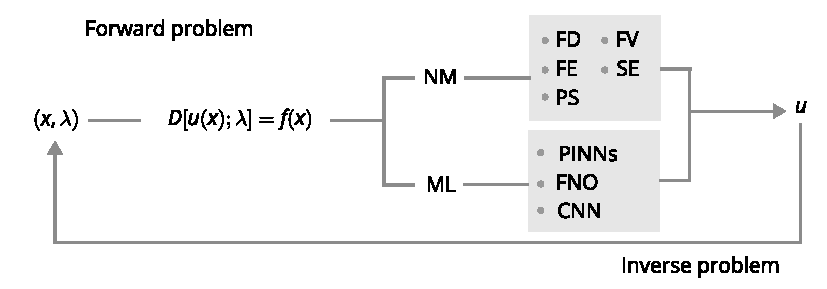
\includegraphics{figs/forward_inverse.pdf}
%     \caption{Scheme of the forward and inverse problems encountered in solving partial differential equations (PDEs). In the forward scenario, the inputs $(x,\lambda)$ are employed to characterize a model across PDEs. Subsequently, the PDEs are resolved through either numerical methods (NM) or machine learning (ML) to derive a solution $u$. Numerical methods encompass finite differences (FD), finite elements (FE), pseudo-spectral (PS), finite volumes (FV), and spectral elements (SE). Machine learning techniques include Physics Informed Neural Networks (PINNs), Fourier Neural Operator (FNO), and Convolutional Neural Networks (CNN). In the case of the inverse problem, the objective is to determine the parameters $(x,\lambda)$ starting from the solution $u$.}
%     \label{fig:forward_inverse}
% \end{figure*}

% \section{Numeric methods to solve the wave propagation problem}

% \subsection{Finite-differences method formulation}

% The finite-difference method is among the most popular to solve partial differential equations, and particularly the wave equation. A complete review of the finite-differences method applied to wave propagation can be found the \citet{Moczo2014} and \citet{Seriani2020}. Partial derivatives are approximated by discrete operators involving differences between adjacent grid points. The derivative of a function $f$ is defined as:\\

% \begin{center}
% $
% \frac{df}{dx} = \lim_{dx \rightarrow 0} \frac{f(x + dx)-f(x)}{dx}
% $ , $
% \frac{df}{dx} = \lim_{dx \rightarrow 0} \frac{f(x + dx)-f(x -dx)}{2dx}
% $ or $
% \frac{df}{dx} = \lim_{dx \rightarrow 0} \frac{f(x)-f(x -dx)}{2dx} \ .
% $
% \end{center}


% Considering the Taylor series expansion:



% Then, the approximation schemes of finite-difference derivative, using the Taylor series expansion, are:\\

% \begin{center}
% $
% \frac{df}{dx}^{+} \approx \frac{f(x + dx)-f(x)}{dx}
% $ , $
% \frac{df}{dx}^{c} \approx  \frac{f(x + dx)-f(x -dx)}{2dx}
% $ and $
% \frac{df}{dx}^{-} \approx \frac{f(x)-f(x -dx)}{2dx}
% $
% \end{center}

% Also, the second-order approximation:\

% $$
% \frac{d^{2}f}{dx^{2}} \approx \frac{f(x+dx)-2f(x)+f(x -dx)}{dx} \ .  
% $$

% \

% The following notation is considered for the discrete case of spatial and temporal variables:\

% $$
% u(x,t) \rightarrow u_{j}^{n}
% $$

% \


%  which is also called an \emph{structured grid}. Thus, equation \ref{scalar} can be expressed as:\\

%  $$
% \frac{u_{j}^{n+1} - 2 u_{j}^{n} + u_{j}^{n-1}}{dt^2} = c_{j}^2 \left[ \frac{u_{j}^{n+1} - 2 u_{j}^{n} + u_{j}^{n-1}}{dx^2} \right]  + s_{j}^n
%  $$

% then,

% $$
% u_{j}^{n+1} = \left( c_{j} \frac{dt}{dx} \right)^2 \left[ u_{j+1}^{n} - 2 u_{j}^{n} + u_{j-1}^{n}\right] + 2 u_{j}^{n} - u_{j}^{n-1} + dt^{2} s_{j}^{n}
% $$


% \


% To model this case, a source point is considered, as

% $$
% s(x, t) = \delta(x - x_s) \cdot f(t)
% $$

% Finite-difference methods fall into two broad categories: explicit and implicit. Explicit schemes for simulating the wave equation determine the motion at a spatial location at a future time exclusively from the motion already calculated for previous times. On the other hand, implicit schemes simultaneously determine the motion at all spatial locations at a future time from known values at previous times using a matrix inversion technique.

% In wave propagation simulations, the partial differential equations are typically discretized on a staggered grid \cite{Virieux1986}. This approach facilitates the resolution of the rupture propagation problem. Particularly an approach was proposed in the work of \citet{Zhou2021} a finite-difference method with variable-length temporal and spatial operators was proposed to increase the stability and efficiency of the traditional method.

% \citet{liu_simulation_2023} combined a standard staggered-grid (SSG), finite-difference (FD) approach and the perfectly matched layer (PML) absorbing boundary to solve 3D first-order velocity-stress equations of acoustoelasticity to simulate wave propagating.

% %----------------------------
% \subsection{Pseudo-spectral method formulation}



 
% %----------------------------
% \subsection{Finite-elements method formulation}


% Finite-element methods are suitable for dealing with intricate shapes and diverse materials because they can use irregular grids. They permit flexibility in size, shape, and approximation order. Nevertheless, a drawback is their high demand for computing power \cite{Padovani,seron-1990}. This methodology involves the transformation of the problem at hand into a system of linear equations utilizing the weak formulation of the pertinent differential equation. This transformation is facilitated by employing an interpolation basis comprised of polynomials defined over disjoint domains, commonly referred to as elements.\\

% The finite-element discretization technique, usually denoted as the semidiscrete Galerkin
% formulation, reduces the seismic modeling problem to the following system of second-order, linear, ordinary differential equations:


% \begin{align}
% M\ddot{u} + K u &= \hat{f} \quad \text{for } t \in (0, T) \notag\\
% u(0) &= u_0 \label{fd-formulation-no-damption}\\
% \dot{u}(0) &= \dot{u}_0 \notag
% \end{align}

% where $M$ is the mass matrix, $K$ is the stiffness matrix, $f$ is the load vector and $u$ is the displacement vector.

% One of the problems arising in numerically modeling wave propagation on the earth is the
% need to use a bounded domain which generates undesired reflections. One way to avoid these
% artifacts is to use a very large domain, but this solution is in practice prevented because it requires huge computer storage. To eliminate unwanted reflections we introduce a damping term $A(x,y,z) u$ for $i = 1,2,3$ in differential equation \ref{fd-formulation-no-damption} which is defined only on a boundary layer surrounding the domain. This method can be very accurate but one needs to adjust the damping term.
% The semidiscrete Galerkin formulation, including the damping term, is

% \begin{align}
% M\ddot{u} + C u + K u &= \hat{f} \quad \text{for } t \in (0, T) \notag\\
% u(0) &= u_0 \\
% \dot{u}(0) &= \dot{u}_0 \notag
% \end{align}

% where the damping matrix $C$ is also sparse, symmetric and positive-definite.

% SolidsPy, an open-source software developed by \citet{solidspy}, employs finite element analysis to tackle 2D elasticity problems. It serves as a valuable tool for researchers in computational mechanics and students in Computational Modeling courses, while also finding applications in graduate courses introducing the Finite Element Method. Similarly, FEniCS, proposed by \citet{FEniCS}, offers a computing platform specifically designed for solving partial differential equations using the finite element method.

% %----------------------------
% \section{Machine learning as an alternative to traditional methods}


% Thanks to the great progress of artificial intelligence, in particular machine learning, many scientists start to explore the potential of using ML to address problems such as mechanical wave propagation. As we have presented the classical numerical methods have achieve high accuracy in their solutions. However, the can be considered computationally expensive when applied to the inverse problem. 


% In recent years, machine learning methods have emerged as an attractive tool to enrich and complement traditional methods, thus allowing challenges to be addressed on multiple dimensions, scales and parameterizations with the promise of efficiency and precision. For example, researchers have explored the Fourier Neural Operator for both forward and inverse analysis of the 2D acoustic wave equation. However, these studies depend on extensive sets of high-quality labeled data, which can be challenging to generate or obtain. There is a critical need to innovate machine learning methods that can effectively handle imperfect measurement data, such as sparse and potentially noisy datasets.\cite{li_fourier_2021}


% \subsection{Convolutional Neural Networks}


% \subsection{Fourier Neural Operator}


% \subsection{Physics-informed neural network}

% Particularly, there has been an increasing interest in leveraging physics-informed neural networks (PINNs) since the published work of \citet{Raissi2019} and \citet{karniadakis_physics-informed_2021}. Although similar ideas for constraining neural networks using physical laws have been explored in previous studies.\cite{lagaris_artificial_1998}


% While PINNs have demonstrated success in diverse scientific problems, it is essential to highlight their limited competence compared to traditional numerical methods in terms of solution accuracy for  simulations.\cite[2.54cm]{moseley_physics-informed_2022} 

% \begin{table}[h]
%     \centering
%     \label{tab:algorithm-pinns}
%     \begin{tabular}{|c|p{0.7\textwidth}|}
%     \hline
%     \textbf{Step} & \textbf{Description} \\ \hline
%     1 & Define the training set domain, governing physical formula, and initial/boundary conditions. \\ \hline
%     2 & Initialize the parameters for the approximator network. \\ \hline
%     3 & Compute approximate solution \(u(x, t)\). \\ \hline
%     4 & Compute the residual loss by calculating the physical loss and initial and boundary condition losses. \\ \hline
%     5 & Use the residual loss to train the approximator network and optimize its parameters \(\theta\) (and \(\eta\) if is also to be inferred) by minimizing the residual loss value. \\ \hline
%     6 & Repeat steps (3-5) until reaching a halt threshold. \\ \hline
%     \end{tabular}
%     \caption[][2cm]{Algorithm of Physics-informed neural network for solving the wave PDE.}
% \end{table}

% Alternative machine learning approaches for predicting physical systems employ various algorithms of machine learning, being the lack of interpretability and the huge amount of data required common disadvantages. In most cases, machine learning learning algorithms are assumed as a black box.


% A notable advantage of PINNs method lies in its ability to formulate tailored loss and activation functions derived from the implemented physical model.\cite{Raissi2019}

% Their significant potential lies in addressing surrogate modeling and inverse analysis, striking a balance between accuracy and computational efficiency.\cite{Song2022}

% The method have shown effectiveness in inverse problems in the context of acoustic wave equations.%\cite{rash_2022}

% PINNs aim to address physical systems governed by the equation
% \[
% N[u(t, x); \lambda] = 0,
% \]
% where \(x \in \mathbb{R}^D\) and \(t \in \mathbb{R}\). The expression \(N[u(t, x); \lambda]\) denotes an underlying differential operator that characterizes the physical system, parametrized by \(\lambda\). The function \(u(t, x)\) represents the system's solution.

% The introduction of PINNs has generated a large amount of work related. For example the work of \cite{karimpouli_physics_2020} explores the application of deep learning in geosciences, specifically solving the 1-dimensional time-dependent seismic wave equation. Comparing Gaussian process and physics-informed neural networks, the research shows that these meshless methods, requiring smaller datasets, effectively incorporate physics laws, with Gaussian process excelling in solution prediction and the neural network proving superior in velocity and density inversion.


% In , PINNs were successfully applied to the 2D acoustic wave equation, demonstrating satisfactory outcomes in forward wave propagation and full waveform inversions (FWIs), despite the efficiency of traditional methods. Additionally, PINNs showcased efficient performance in solving the inverse problem. Similarly, in \cite{ren_seismicnet_2024}, PINNs were employed for modeling mechanical wave propagation in semi-infinite domains, showcasing their versatility in forward modeling for seismic wave propagation, without requiring labeled data. These studies collectively highlight the effectiveness of PINNs across different wave propagation scenarios.
